\documentclass[11pt]{article}

\usepackage{fancybox}



\usepackage{color}
\usepackage{url}
\usepackage[margin=1in]{geometry}


\renewcommand{\textfraction}{0.0}
\renewcommand{\topfraction}{1.0}
%\renewcommand{\textfloatsep}{5mm}


% Definitions of handy macros can go here
\usepackage{amsmath,amssymb,amsthm,bm,mathtools}
\usepackage{mathrsfs}

\usepackage{multirow}
\usepackage{natbib}
%\usepackage{dsfont,multirow,hyperref,setspace,natbib,enumerate}
\usepackage{dsfont,multirow,hyperref,setspace,enumerate}
\hypersetup{colorlinks,linkcolor={blue},citecolor={blue},urlcolor={red}}
\usepackage{algpseudocode,algorithm}
\algnewcommand\algorithmicinput{\textbf{Input:}}
\algnewcommand\algorithmicoutput{\textbf{Output:}}
\algnewcommand\INPUT{\item[\algorithmicinput]}
\algnewcommand\OUTPUT{\item[\algorithmicoutput]}

\mathtoolsset{showonlyrefs=true}



\theoremstyle{plain}
\newtheorem{thm}{Theorem}[section]
\newtheorem{lem}{Lemma}[section]
\newtheorem{prop}{Proposition}[section]
\newtheorem{pro}{Property}[section]
\newtheorem{assumption}{Assumption}[section]

\theoremstyle{definition}
\newtheorem{defn}{Definition}[section]
\newtheorem{cor}{Corollary}[section]
\newtheorem{example}{Example}[section]
\newtheorem{rmk}{Remark}[section]


\renewcommand{\thefigure}{{S\arabic{figure}}}%
\renewcommand{\thetable}{{S\arabic{table}}}%
\renewcommand{\figurename}{{Supplementary Figure}}
\renewcommand{\tablename}{{Supplementary Table}}
\setcounter{figure}{0}
\setcounter{table}{0}


\def\MLET{\hat \Theta_{\text{MLE}}}
\newcommand{\cmt}[1]{{\leavevmode\color{red}{#1}}}



\usepackage{dsfont}

\usepackage{multirow}

\DeclareMathOperator*{\minimize}{minimize}

\usepackage{wrapfig}

\usepackage{mathtools}
\usepackage{enumitem}
\mathtoolsset{showonlyrefs}
\newcommand*{\KeepStyleUnderBrace}[1]{%f
  \mathop{%
    \mathchoice
    {\underbrace{\displaystyle#1}}%
    {\underbrace{\textstyle#1}}%
    {\underbrace{\scriptstyle#1}}%
    {\underbrace{\scriptscriptstyle#1}}%
  }\limits
}
\usepackage{xr}
\externaldocument{signT_v1}
\input macros.tex
\usepackage{comment}


\def\sign{\textup{sgn}}
\def\srank{\textup{srank}}
\def\rank{\textup{rank}}
\def\caliP{\mathscr{P}_{\textup{sgn}}}
\def\risk{\textup{Risk}}
\usepackage{microtype}

\title{Supplements for ``Beyond the Signs: Nonparametric Tensor Completion via Sign Series''}


\begin{document}

\begin{center}
\begin{spacing}{1.5}
\textbf{\Large Appendix for ``Beyond the Signs: Nonparametric Tensor Completion via Sign Series''}
\end{spacing}
\end{center}

\appendix
The appendix consists of proofs (Section~\ref{sec:proof}), additional theoretical results (Section~\ref{sec:additional}),  and numerical experiments (Section~\ref{sec:data}).


\section{Proofs}\label{sec:proof}
\subsection{Proofs of Propositions~\ref{cor:monotonic}-\ref{prop:global}}
\begin{proof}[Proof of Proposition~\ref{cor:monotonic}]
The strictly monotonicity of $g$ implies that the inverse function $g^{-1}\colon \mathbb{R}\to \mathbb{R}$ is well-defined. 
When $g$ is strictly increasing, the mapping $x\mapsto g(x)$ is sign preserving. Specifically, if $x\geq 0$, then $g(x)\geq g(0)=0$. Conversely, if $g(x)\geq 0=g(0)$, then applying $g^{-1}$ to both sides gives $x\geq 0$.
When $g$ is strictly decreasing, the mapping $x\mapsto g(x)$ is sign reversing. Specifically, if $x\geq 0$, then $g(x)\leq g(0)=0$. Conversely, if $g(x)\geq 0=g(0)$, then applying $g^{-1}$ to both sides gives $x\leq 0$.
 Therefore, $\Theta\simeq g(\Theta)$,  or $\Theta\simeq -g(\Theta)$. Since constant multiplication  does not change the tensor rank,  we have $\srank(\Theta)=\srank(g(\Theta))\leq \rank (g(\Theta))$. 
\end{proof}


\begin{proof}[Proof of Proposition~\ref{cor:broadness}]
See Section~\ref{sec:high-rank} for constructive examples.
\end{proof}

\begin{proof}[Proof of Proposition~\ref{prop:global}]
Fix $\pi\in[-1,1]$. Based on the definition of classification loss $L(\cdot,\cdot)$, the function $\risk(\cdot)$ relies only on the sign pattern of the tensor. Therefore, without loss of generality, we assume both $\bar \Theta, \tZ \in\{-1,1\}^{d_1\times \cdots \times d_K}$ are binary tensors. 
We evaluate the excess risk 
\begin{equation}\label{eq:risk}
\risk(\tZ)- \risk(\bar \Theta) = \mathbb{E}_{\omega\sim \Pi}\KeepStyleUnderBrace{\mathbb{E}_{\tY(\omega)}\left\{|\tY(\omega)-\pi|\left[\left|\tZ(\omega)-\sign(\bar \tY(\omega)) \right|-\left|\bar\Theta(\omega)-\sign(\bar \tY(\omega))\right|\right]\right\}}_{\stackrel{\text{def}}{=}I(\omega)}.
\end{equation}
Denote $y=\tY(\omega)$, $z=\tZ(\omega)$, $\bar \theta=\bar\Theta(\omega)$, and $\theta=\Theta(\omega)$. The expression of $I(\omega)$ is simplified as
\begin{align}\label{eq:I}
I(\omega)&= \mathbb{E}_{y}\left[ (y-\pi)(\bar \theta-z)\mathds{1}(y\geq \pi)+(\pi-y)(z-\bar \theta)\mathds{1}(y< \pi)\right]\notag \\
&= \mathbb{E}_{y}\left[(\bar \theta-z) (y-\pi)\right]\notag \\
&=  \left[\sign(\theta-\pi)-z\right]\left(\theta-\pi\right)\notag \\
&= |\sign(\theta-\pi)-z||\theta-\pi|\geq 0,
\end{align}
where the third line uses the fact $\mathbb{E}y=\theta$ and $\bar \theta=\sign(\theta-\pi)$, and the last line uses the assumption $z \in\{-1,1\}$. The equality~\eqref{eq:I} is attained when $z=\sign(\theta-\pi)$ or $\theta=\pi$. Combining~\eqref{eq:I} with~\eqref{eq:risk}, we conclude that, for all $\tZ\in\{-1,1\}^{d_1\times \cdots \times d_K}$, 
\begin{equation}\label{eq:minimum}
\risk(\tZ)- \risk(\bar \Theta) = \mathbb{E}_{\omega\sim \Pi} |\sign(\Theta(\omega)-\pi)-\tZ(\omega)||\Theta(\omega)-\pi|\geq 0,
\end{equation}
In particular, setting $\tZ=\bar \Theta=\sign(\Theta-\pi)$ in~\eqref{eq:minimum} yields the minimum. Therefore, 
\[
\risk(\bar \Theta)=\min\{\risk(\tZ)\colon \tZ\in \mathbb{R}^{d_1\times \cdots \times d_K}\} \leq \min\{\risk(\tZ)\colon \rank(\tZ)\leq r\}.
\]
Since $\srank(\Theta-\pi)\leq r$ by assumption, the last inequality becomes equality. The proof is complete. 
\end{proof}

\subsection{Proof of Theorem~\ref{thm:population}}
\begin{proof}[Proof of Theorem~\ref{thm:population}]
Fix $\pi\in[-1,1]$. Based on~\eqref{eq:minimum} in Proposition~\ref{prop:global} we have
\begin{equation}\label{eq:population2}
\risk(\tZ)- \risk(\bar \Theta) = \mathbb{E}\left[|\sign \tZ-\sign\bar \Theta||\bar \Theta|\right].
\end{equation}
The Assumption~\ref{ass:margin} states that
\begin{equation}\label{eq:ass}
\mathbb{P}\left(|\bar \Theta | \leq t\right)\leq ct^\alpha,\quad \text{for all } 0\leq t< \rho(\pi,\tN).
\end{equation}
Without future specification, all relevant probability statements, such as $\mathbb{E}$ and $\mathbb{P}$, are with respect to $\omega\sim \Pi$. 

We divide the proof into two cases: $\alpha >0$ and $\alpha = \infty$.
\begin{itemize}[leftmargin=*,topsep=0pt,itemsep=-1ex,partopsep=1ex,parsep=1ex]
\item Case 1: $\alpha>0$. 

By~\eqref{eq:population2}, for all $0\leq t< \rho(\pi, \tN)$,
\begin{align}\label{eq:1}
\risk(\tZ)- \risk(\bar \Theta) &\geq t\mathbb{E}\left(|\sign \tZ- \sign \hat\Theta|\mathds{1}\{|\hat\Theta|>t\}\right)
\notag \\
&\geq 2t\mathbb{P}\left(\sign\tZ \neq \sign \bar \Theta\text{ and }|\bar \Theta|>t   \right)\notag \\
& \geq 2t\Big\{\mathbb{P}\left(\sign\tZ \neq \sign \bar \Theta \right) - \mathbb{P}\left(|\bar \Theta|\leq t\right)\Big\}\notag\\
&\geq t\Big\{\textup{MAE}(\sign \tZ, \sign \bar \Theta) - 2ct^\alpha \Big\},
\end{align}
where the last line follows from the definition of MAE and~\eqref{eq:ass}. We maximize the lower bound~\eqref{eq:1} with respect to $t$, and obtain the optimal $t_{\text{opt}}$,
\[
t_{\text{opt}}=\begin{cases}
\rho(\pi, \tN), & \text{if } \textup{MAE}(\sign \tZ,\sign \bar\Theta) > 2c(1+\alpha) \rho^{\alpha}(\pi, \tN),\\
\left[ {1\over 2c(1+\alpha)} \textup{MAE} (\sign \tZ,\sign \bar\Theta)  \right]^{1/\alpha}, &  \text{if }\textup{MAE}( \sign \tZ,\sign \bar\Theta) \leq 2c(1+\alpha) \rho^{\alpha}(\pi, \tN).
 \end{cases}
\]
The corresponding lower bound of the inequality~\eqref{eq:1} becomes
\[
\risk(\tZ)- \risk(\bar \Theta) \geq 
\begin{cases}
c_1 \rho(\pi, \tN) \textup{MAE}(\sign \tZ,\sign \bar\Theta),  & \text{if } \textup{MAE}(\sign \tZ,\sign \bar\Theta) > 2c(1+\alpha) \rho^{\alpha}(\pi, \tN),\\
c_2 \left[ \textup{MAE}( \sign \tZ,\sign \bar\Theta)\right]^{1+\alpha \over \alpha}, & \text{if }\textup{MAE}(\sign \tZ,\sign \bar\Theta) \leq 2c(1+\alpha) \rho^{\alpha}(\pi, \tN),
\end{cases}
\]
where $c_1,c_2>0$ are two constants independent of $\tZ$. Combining both cases gives
\begin{align}\label{eq:MAE}
\textup{MAE}(\sign \tZ,\sign \bar\Theta) & \lesssim [\risk(\tZ)- \risk(\bar \Theta)]^{\alpha\over 1+\alpha}+{1\over \rho(\pi, \tN)} \left[\risk(\tZ)- \risk(\bar \Theta)\right]\\
&\leq C(\pi)[\risk(\tZ)- \risk(\bar \Theta)]^{\alpha\over 1+\alpha},
\end{align}
where $C(\pi)>0$ is a multiplicative factor independent of $\tZ$. 
\item Case 2: $\alpha=\infty$. The inequality~\eqref{eq:1} now becomes
\begin{equation}\label{eq:2}
\risk(\tZ)- \risk(\bar \Theta) \geq t\textup{MAE}(\sign \bar\Theta, \sign \tZ), \quad \text{for all }0\leq t< \rho(\pi,\tN).
\end{equation}
The conclusion follows by taking $t={\rho(\pi, \tN)\over 2}$ in the inequality~\eqref{eq:2}. 
\end{itemize}
\end{proof}
\begin{rmk}\label{eq:rmk}The proof of Theorem~\ref{thm:population} shows that, under Assumption~\ref{ass:margin}, 
\begin{equation}\label{eq:remark}
\textup{MAE}(\sign \tZ,\sign \bar \Theta)  \lesssim [\risk(\tZ)- \risk(\bar \Theta)]^{\alpha\over 1+\alpha}+{1\over \rho(\pi, \tN)} \left[\risk(\tZ)- \risk(\bar \Theta)\right],
\end{equation}
for all $\tZ\in\mathbb{R}^{d_1\times \cdots \times d_R}$. For fixed $\pi$, the second term is absorbed into the first term. 
\end{rmk}

\subsection{Proof of Theorem~\ref{thm:classification}}
The following lemma provides the variance-to-mean relationship implied by the $\alpha$-smoothness of $\Theta$. The relationship plays a key role in determining the convergence rate based on empirical process theory~\citep{shen1994convergence}. 
\begin{lem}[Variance-to-mean relationship]\label{lem:variance}
Consider the same setup as in Theorem~\ref{thm:classification}. Fix $\pi\in[-1,1]$. Let $L(\tZ, \bar Y_\Omega)$ be the $\pi$-weighted classification loss
\begin{align}\label{eq:sample2}
L(\tZ, \bar \tY_\Omega)&= {1\over |\Omega|}\sum_{\omega \in \Omega}\ \KeepStyleUnderBrace{|\bar \tY(\omega)|}_{\text{weight}}\  \times \ \KeepStyleUnderBrace{| \sign \tZ(\omega)-\sign \bar \tY(\omega)|}_{\text{classification loss}}\notag \\
&={1\over |\Omega|}\sum_{\omega \in \Omega}\ell_\omega(\tZ, \bar \tY),
\end{align}
where we have denoted the function $\ell_\omega(\tZ,\bar \tY)\stackrel{\text{def}}{=}|\bar \tY(\omega)||\sign\tZ(\omega)-\sign \bar \tY(\omega)|$. Under Assumption~\ref{ass:margin} of the $(\alpha,\pi)$-smoothness of $\Theta$, we have
\begin{equation}\label{eq:variance}
\textup{Var}[\ell_\omega(\tZ,\bar \tY)-\ell_\omega(\bar \Theta, \bar \tY_\Omega)]\lesssim [\textup{Risk}(\tZ)-\textup{Risk}(\bar \Theta)]^{\alpha \over 1+\alpha}+{1\over \rho(\pi, \tN)}[\textup{Risk}(\tZ)-\textup{Risk}(\bar \Theta)],
\end{equation}
for all tensors $\tZ\in\mathbb{R}^{d_1\times \cdots \times d_K}$. Here the expectation and variance are taken with respect to both $\tY$ and $\omega\sim \Pi$. 
\end{lem}
\begin{proof}[Proof of Lemma~\ref{lem:variance}]
We expand the variance by
\begin{align}\label{eq:mae}
\text{Var}[\ell_\omega(\tZ,\bar \tY_\Omega)-\ell_\omega(\bar \Theta, \bar \tY_\Omega)] &\lesssim \mathbb{E}|\ell_\omega(\tZ,\bar \tY_\Omega)-\ell_\omega(\bar \Theta, \bar \tY_\Omega)|^2\notag \\
&\lesssim \mathbb{E}|\ell_\omega(\tZ,\bar \tY_\Omega)-\ell_\omega(\bar \Theta, \bar \tY_\Omega)|\notag \\
&\leq \mathbb{E}|\sign\tZ-\sign \bar \Theta| = \textup{MAE}(\sign\tZ, \sign \bar \Theta),
\end{align}
where the second line comes from the boundedness of classification loss $L(\cdot ,\cdot)$, and the third line comes from the inequality $||a-b|-|c-b||\leq |a-b|$ for $a,b,c\in\{-1,1\}$, together with the boundedness of classification weight $|\bar\tY(\omega)|$. Here we have absorbed the constant multipliers in $\lesssim$. The conclusion~\eqref{eq:variance} then directly follows by applying Remark~\ref{eq:rmk} to~\eqref{eq:mae}.
\end{proof}

\begin{proof}[Proof of Theorem~\ref{thm:classification}]
Fix $\pi\in[-1,1]$. For notational simplicity, we suppress the subscript $\pi$ and write $\hat \tZ$ in place of $\hat \tZ_\pi$. Denote $n=|\Omega|$ and $\rho=\rho(\pi, \tN)$. 

Because the classification loss $L(\cdot, \cdot)$ is scale-free, i.e., $L(\tZ,\cdot)=L(c\tZ, \cdot)$ for every $c>0$, we consider the estimation subject to $\FnormSize{}{\tZ}\leq 1$ without loss of generality. Specifically, let
\[
\hat \tZ=\argmin_{\tZ\colon \textup{rank}(\tZ)\leq r, \FnormSize{}{\tZ}\leq 1}L(\tZ, \bar \tY_{\Omega}).
\]

We next apply the empirical process theory to bound $\hat \tZ$. To facilitate the analysis, we view the data $\bar \tY_\Omega=\{\bar \tY(\omega)\colon \omega\in \Omega\}$ as a collection of $n$ independent random variables where the randomness is from both $\bar \tY$ and $\omega\sim\Pi$. Write the index set $\Omega=\{1,\ldots,n\}$, so the loss function~\eqref{eq:sample2} becomes
\[
L(\tZ,\bar \tY_\Omega)={1\over n}\sum_{i=1}^n\ell_{i}(\tZ, \bar \tY).
\]
We use $f_\tZ \colon [d_1]\times\cdots\times[d_n] \to \mathbb{R}$ to denote the function induced by tensor $\tZ$ such that $f_\tZ(\omega)=\tZ(\omega)$ for $\omega\in[d_1]\times \cdots \times [d_K]$. Under this set-up, the quantity of interest
\begin{align}\label{eq:empirical}
 L(\tZ,\bar \tY_\Omega)-L(\bar \Theta,\bar \tY_\Omega)={1\over n}\sum_{i=1}^n \KeepStyleUnderBrace{\left[\ell_{i}(\tZ, \bar \tY)-\ell_{i}(\bar \Theta, \bar \tY)\right]}_{\stackrel{\text{def}}{=}\Delta_i(f_\tZ,\bar \tY)},
\end{align}
is an empirical process induced by function $f_{\tZ}\in \tF_{\tT}$ where $\tT=\{\tZ\colon \rank(\tZ)\leq r, \ \FnormSize{}{\tZ}\leq 1\}$. Note that there is an one-to-one correspondence between sets $\tF_{\tT}$ and $\tT$. 

Our remaining proof adopts the techniques of~\citet[Theorem 3]{wang2008probability} to bound~\eqref{eq:empirical} over the function family $f_{\tZ}\in \tF_{\tT}$. We summarize only the key difference here but refer to~\cite{wang2008probability} for complete proof. 
Based on Lemma~\ref{lem:variance}, the $(\alpha,\pi)$-smoothness of $\Theta$ implies 
\begin{equation}\label{eq:second}
\textup{Var}\Delta_i(f_\tZ,\bar \tY) \lesssim \left[\mathbb{E}\Delta_i(f_\tZ,\bar \tY)\right]^{\alpha \over 1+\alpha}+{1\over \rho}\mathbb{E}\Delta_i(f_\tZ,\bar \tY),\quad \text{for all $f_\tZ\in \tF_\tT$}.
\end{equation}
Applying local iterative techniques in~\citet[Theorem 3]{wang2008probability} to the empirical process~\eqref{eq:empirical} with the variance-to-mean relationship~\eqref{eq:second} gives that
\begin{equation}\label{eq:rate}
\mathbb{P}\left(\risk(\hat \tZ)-\risk(\bar \Theta )\geq L_n\right)\lesssim \exp(-nL_n),
\end{equation}
where the convergence rate $L_n>0$ is determined by the solution to the following inequality,
\begin{equation}\label{eq:equation}
{1\over L_n}\int_{L_n}^{\sqrt{L_n^{\alpha/(\alpha+1)}+{L_n\over \rho}}}\sqrt{\tH_{[\ ]}(\varepsilon,\tF_{\tT}, \vnormSize{}{\cdot}) }d\varepsilon \leq C\sqrt{n},
\end{equation}
for some constant $C>0$. In particular, the smallest $L_n$ satisfying~\eqref{eq:equation} yields the best upper bound of the error rate. Here $\tH_{[\ ]}(\varepsilon, \tF_{\tT},\vnormSize{}{\cdot})$ denotes the $L_2$-metric, $\varepsilon$-bracketing number (c.f. Definition~\ref{pro:inftynorm}) of family $\tF_{\tT}$. 

It remains to solve for the smallest possible $L_n$ in~\eqref{eq:equation}. Based on Lemma~\ref{lem:metric}, the inequality~\eqref{eq:equation} is satisfied with 
\begin{equation}\label{eq:tn}
L_n\asymp t_n^{(\alpha+1)/ (\alpha+2)} +{1\over \rho} t_n, \quad \text{where }t_n={d_{\max}rK\log K \over n}.
\end{equation}
Therefore, by~\eqref{eq:rate}, with very high probability. 
\[
\risk(\hat \tZ)-\risk(\bar \Theta )\leq t_n^{(\alpha+1)/(\alpha+2)} +{1\over \rho} t_n.
\]
Inserting the above bound into~\eqref{eq:remark} gives
\begin{align}\label{eq:final}
\textup{MAE}(\sign \hat \tZ, \sign \bar \Theta) &\lesssim [\risk(\hat \tZ)-\risk(\bar \Theta)]^{\alpha/(\alpha+1)}+{1\over \rho}[\risk(\hat \tZ)-\risk(\bar \Theta)]\notag \\
&\lesssim t_n^{\alpha/(\alpha+2)}+{1\over \rho^{\alpha/\alpha+1}}t_n^{\alpha/(\alpha+1)}+{1\over \rho}t_n^{(\alpha+1)/(\alpha+2)}+{1\over \rho^2}t_n\notag \\
&\leq 4t_n^{\alpha/(\alpha+2)}+{4\over \rho^2}t_n,
\end{align}
where the last line follows from the fact that $a(b^2+b^{(\alpha+2)/(\alpha+1)}+b+1) \leq 4 a (b^2+1)$ with $a={t_n \over \rho^2}$ and $b=\rho t_n^{-1/(\alpha+2)}$. We plug $t_n$ into~\eqref{eq:final} and absorb the term $K\log K$ into the constant. The conclusion is then proved. 
\end{proof}

\begin{defn}[Bracketing number]\label{pro:inftynorm}
Consider a family of functions $\tF$, and let $\varepsilon>0$. Let $\tX $ denote the domain space equipped with measure $\Pi$. We call $\{(f^l_m,f^u_m)\}_{m=1}^M$ an $L_2$-metric, $\varepsilon$-bracketing function set of $\tF$, if for every $f\in \tF$, there exists an $m\in[M]$ such that 
\[
f^l_m(x)\leq f(x)\leq f^u_m(x),\quad \text{for all }x\in\tX,
\]
and
\[
\vnormSize{}{f^l_m-f^u_m}\stackrel{\text{def}}{=}\sqrt{\mathbb{E}_{x\sim \Pi}|f^l_m(x)-f^u_m(x)|^2} \leq \varepsilon, \ \text{for all } m=1,\ldots,M. 
\]
The bracketing number with $L_2$-metric, denoted $\tH_{[\ ]}(\varepsilon, \tF, \vnormSize{}{\cdot})$, is the logarithm of the smallest cardinality of the $\varepsilon$-bracketing function set of $\tF$.  
\end{defn}



\begin{lem}[Bracketing complexity of low-rank tensors] \label{lem:metric}
Define the family of rank-$r$ bounded tensors $\tT=\{\tZ\in\mathbb{R}^{d_1\times \cdots \times d_K}\colon \rank(\tZ)\leq r, \ \FnormSize{}{\tZ}\leq 1\}$ and the induced function family $\tF_{\tT} = \{f_\tZ\colon \tZ\in\tT\}$.  Set 
\begin{equation}\label{eq:specification}
L_n\asymp \left({d_{\max}rK\log K \over n } \right)^{(\alpha+1)/(\alpha+2)} + {1\over \rho (\pi, \tN)}\left({d_{\max}rK\log K \over n } \right).
\end{equation}
Then, the following inequality is satisfied.
\begin{equation}\label{eq:L}
{1\over L_n}\int^{\sqrt{L_n^{\alpha/(\alpha+1)}+{L_n\over \rho (\pi, \tN)}}}_{L_n} \sqrt{\tH_{[\ ]}(\varepsilon, \tF_{\tT} ,\vnormSize{}{\cdot}) }d\varepsilon \leq Cn^{1/2},
\end{equation}
where $C>0$ is a constant independent of $r,K$  and $d_{\text{max}}$.
\end{lem}
\begin{proof}[Proof of Lemma~\ref{lem:metric}]
To simplify the notation, we denote $\rho=\rho(\pi, \tN)$. 
Notice that 
\begin{align}
	\vnormSize{}{f_{\tZ_1}-f_{\tZ_1}}\leq\|f_{\tZ_1}-f_{\tZ_1}\|_\infty\leq \FnormSize{}{\tZ_1-\tZ_1}\quad\text{ for all } \tZ_1,\tZ_2\in\tT.
\end{align}
It follows from~\citet[Theorem 9.22]{kosorok2007introduction} that the $L_2$-metric, $(2\epsilon)$-bracketing number of $\tF_{\tT}$ is bounded by 
\[
\tH_{[\ ]}(2\varepsilon, \tF_{\tT}, \vnormSize{}{\cdot})\leq \tH(\varepsilon, \tT, \FnormSize{}{\cdot}) \leq Cd_{\max}rK\log {K\over \varepsilon}.
\]
The last inequality is from the covering number bounds for rank-$r$ bounded tensors; see \citet[Lemma 3]{mu2014square}.

Inserting the bracketing number into~\eqref{eq:L} gives
\begin{equation}\label{eq:complexity}
g(L)={1\over L}\int^{\sqrt{L^{\alpha/(\alpha+1)}+{\rho^{-1}L}}}_{L}  \sqrt{d_{\max}rK\log\left({K\over \varepsilon}\right)}d\varepsilon.
\end{equation}
By the monotonicity of the integrand in~\eqref{eq:complexity}, we bound $g(L)$ by 
\begin{align}\label{eq:g}
g(L)&\leq {\sqrt{d_{\max}rK}\over L}\int_{L}^{\sqrt{L^{\alpha/(\alpha+1)}+\rho^{-1}L}}\sqrt{\log \left(K \over L \right)}d\varepsilon\notag \\
&\leq \sqrt{d_{\max}rK(\log K - \log L)}\left({L^{\alpha/(2\alpha+2)}+\sqrt{\rho^{-1}L} \over L }-1\right)\notag \\
&\leq  \sqrt{d_{\max}rK\log K}\left( {1\over L^{(\alpha+2)/(2\alpha+2)}}+{1\over \sqrt{\rho L}}\right),
\end{align}
where the second line follows from $\sqrt{a+b} \leq \sqrt{a}+\sqrt{b}$ for $a,b>0$.
It remains to verify that $g(L_n) \leq Cn^{1/2}$ for $L_n$ specified in~\eqref{eq:L}. Plugging $L_n$ into the last line of~\eqref{eq:g} gives
\begin{align}
g(L_n)&\leq \sqrt{d_{\max}rK\log K}\left( {1\over L_n^{(\alpha+2)/(2\alpha+2)}}+{1\over \sqrt{\rho L_n}}\right)
\\&\leq \sqrt{d_{\max}rK\log K}\left(\left[\left(d_{\max}rK\log K\over n\right)^{\alpha+1\over \alpha+2}\right]^{-{\alpha+2\over2\alpha+2}}+\left[\rho \left(d_{\max}rK\log K\over \rho n\right)\right]^{-{1\over2}} \right)
\\&\leq Cn^{1/2},
\end{align}
where $C>0$ is a constant independent of $r,K$  and $d_{\text{max}}$. The proof is therefore complete.  
\end{proof}

\subsection{Proof of Theorem~\ref{thm:estimation}}
\begin{proof}[Proof of Theorem~\ref{thm:estimation}]
By definition of $\hat\Theta$, we have
\begin{align}\label{eq:pfmain3}\nonumber
\text{MAE}(\hat\Theta,\Theta) &= \mathbb{E}\left|\frac{1}{2H+1}\sum_{\pi\in\Pi}\sign\hat Z_\pi-\Theta\right|\\\nonumber
&\leq \mathbb{E}\left|\frac{1}{2H+1}\sum_{\pi\in\Pi}\left(\sign\hat Z_\pi-\sign(\Theta-\pi)\right)\right|+\mathbb{E}\left|\frac{1}{2H+1}\sum_{\pi\in\Pi}\sign(\Theta-\pi)-\Theta\right|\\&
\leq \frac{1}{2H+1}\sum_{\pi\in\Pi}\text{MAE}(\sign\hat Z_\pi,\sign(\Theta-\pi))+\frac{1}{H},
\end{align}
where the last line comes  from the triangle inequality and the inequality
\begin{equation}
\left|\frac{1}{2H+1}\sum_{\pi\in\Pi}\sign(\Theta(\omega)-\pi)-\Theta(\omega)\right|\leq \frac{1}{H},\quad\text{for all } \omega\in[d_1]\times\cdots\times [d_K].
\end{equation}
Write $n=|\Omega|$. Now it suffices to bound  the first term in \eqref{eq:pfmain3}.  We prove that 
\begin{equation}\label{eq:total}
{1\over 2H+1}\sum_{\pi \in \Pi} \textup{MAE}(\sign \hat Z_\pi, \sign (\Theta-\pi)) \lesssim  t_n^{\alpha/(\alpha+2)}+{1\over H}+ H t_n, \quad \text{with } t_n={d_{\max}rK\log K\over n}.
\end{equation}
Theorem~\ref{thm:classification} implies that the  sign estimation accuracy depends on the closeness of $\pi\in \tH$ to the mass points in $\tH$. Therefore, we partition the level set $\pi \in \tH$ based on their closeness to $\tH$. Specifically, let $\tN_H \stackrel{\text{def}}{=}\bigcup_{\pi'\in\tN}\left(\pi'-\frac{1}{H},\pi'+\frac{1}{H}\right)$ denote the set of levels at least $1\over H$-close to the mass points. We expand~\eqref{eq:total} by
\begin{align}\label{eq:twobounds}
&{1\over 2H+1}\sum_{\pi \in \Pi} \textup{MAE}(\sign \hat Z_\pi, \sign (\Theta-\pi))\notag \\
=&{1\over 2H+1}\sum_{\pi \in \Pi\cap \tN_H} \textup{MAE}(\sign \hat Z_\pi, \sign (\Theta-\pi))+{1\over 2H+1}\sum_{\pi \in \Pi\cap \tN_H^c} \textup{MAE}(\sign \hat Z_\pi, \sign (\Theta-\pi)).
\end{align}
By assumption, the first term involves only finite number of summands and thus can be bounded by $4C/ (2H+1)$ where $C>0$ is a constant such that $|\tN|\leq C$.  We bound the second term using the explicit forms of $\rho(\pi, \tN)$ in the sequence $\pi \in\Pi\cap \tN_H^c$. Based on Theorem~\ref{thm:classification}, 
\begin{align}
{1\over 2H+1}\sum_{\pi \in \Pi\cap \tN_H^c} \textup{MAE}(\sign \hat \tZ_\pi, \sign (\Theta-\pi)) &\lesssim  {1\over 2H+1}\sum_{\pi\in \Pi\cap \tN_H^c} t_n^{\alpha/(\alpha+2)}+{t_n\over 2H+1}\sum_{\pi \in \Pi\cap \tN_H^c}{1\over \rho^2(\pi, \tN)}\\
&\leq t_n^{\alpha/(\alpha+2)}+{t_n\over 2H+1} \sum_{\pi \in \Pi\cap \tN_H^c} \sum_{\pi' \in \tN}{1\over |\pi-\pi'|^2}\\
&\leq  t_n^{\alpha/(\alpha+2)}+{t_n\over 2H+1} \sum_{\pi'\in \tN} \sum_{\pi \in \Pi\cap \tN_H^c}{1\over |\pi-\pi'|^2}\\
&\leq t_n^{\alpha/(\alpha+2)}+ 2CHt_n,
\end{align}
where the last inequality follows from the Lemma~\ref{lem:H}.  Combining the bounds for the two terms in \eqref{eq:twobounds} completes the proof for conclusion~\eqref{eq:total}. Finally, plugging \eqref{eq:total} into \eqref{eq:pfmain3} yields
\begin{align}
\text{MAE}(\hat\Theta,\Theta)\lesssim \left(d_{\max}rK\log K\over |\Omega|\right)^{\alpha/(\alpha+2)}+\frac{1}{H}+H{d_{\max}rK\log K\over |\Omega|}.
 \end{align}
The conclusion follows by absorbing $K\log K$ into the constant term in the statement. 
\end{proof}


\begin{lem}\label{lem:H}
Fix $\pi'\in\tN$ and a sequence $\Pi=\{-1,\ldots,-1/H,0,1/H,\ldots,1\}$ with $H\geq 2$. Then, 
\[
\sum_{\pi \in \Pi\cap \tN_H^c}{1\over 
|\pi-\pi'|^2}\leq 4H^2. 
\]
\begin{proof}[Proof of Lemma~\ref{lem:H}]
Notice that all points $\pi\in\Pi\cap\tN_H^c$ satisfy $|\pi-\pi'|>{1\over H}$ for all $\pi'\in\tN$. We use this fact to compute the sum
\begin{align}
   \sum_{\pi \in \Pi\cap \tN_H^c}{1\over |\pi-\pi'|^2}&= \sum_{\frac{h}{H}\in\Pi\cap \tN_H^c } {1\over |\frac{h}{H}-\pi'|^2}\\
   &\leq 2H^2\sum_{h=1}^{H}{1 \over h^2}\\
 &\leq 2H^2\left\{ 1+\int_{1}^2{1\over x^2}dx+ \int_{2}^3{1\over x^2}dx+\cdots + \int_{H-1}^H{1\over x^2}dx\right\}\\
&= 2H^2\left(1+\int^{H}_{1}{1\over x^2}dx\right) \leq 4H^2,
\end{align}
 where the third line uses the monotonicity of ${1\over x^2}$ for $x\geq 1$. 
 \end{proof}
\end{lem}


\section{Additional results}\label{sec:additional}
\subsection{Sensitivity of tensor rank to monotonic transformations}
In Section~\ref{sec:intro} of the main paper, we have provided a motivating example to show the sensitivity of tensor rank to monotonic transformations. Here, we describe the details of the example set-up. 

The step 1 is to generate a rank-3 tensor $\tZ$ based on the CP representation
\[
\tZ=\ma^{\otimes 3}+\mb^{\otimes 3}+\mc^{\otimes 3},
\]
where $\ma,\mb,\mc\in\mathbb{R}^{30}$ are vectors consisting of $N(0,1)$ entries, and the shorthand $\ma^{\otimes 3}=\ma\otimes \ma\otimes \ma$ denotes the Kronecker power. We then apply $f(z)=(1+\exp(-cz))^{-1}$ to $\tZ$ entrywise, and obtain a transformed tensor $\Theta=f(\tZ)$. 

The step 2 is to determine the rank of $\Theta$. Unlike matrices, the exact rank determination for tensors is NP hard. Therefore, we choose to compute the numerical rank of $\Theta$ as an approximation.  The numerical rank is determined as the minimal rank for which the relative approximation error is below $0.1$, i.e.,
\begin{equation}\label{eq:numeric}
 \hat r(\Theta)=\min\left\{s\in\mathbb{N}_{+}\colon \min_{\hat \Theta\colon \rank(\hat \Theta)\leq s}{\FnormSize{}{\Theta-\hat \Theta}\over \FnormSize{}{\Theta}} \leq 0.1\right\}.
\end{equation}
We compute $\hat r(\Theta)$ by searching over $s\in\{1,\ldots,30^2\}$, where for each $s$, we (approximately) solve the least-square minimization using CP function in R package {\tt rTensor}. 
We repeat steps 1-2 ten times, and plot the averaged numerical rank of $\Theta$ versus transformation level $c$ in Figure~\ref{fig:example}a.  

\subsection{Tensor rank and sign-rank}\label{sec:high-rank}
In the main paper, we have provided several tensor examples with high tensor rank but low sign-rank. This section provides more examples and their proofs. 
Unless otherwise specified, let $\Theta$ be an order-$K$ $(d,\ldots,d)$-dimensional tensor. 
\begin{example}[Max hypergraphon]\label{example:max} Suppose the tensor $\Theta$ takes the form 
\[
\Theta(i_1,\ldots,i_K)=\log\left(1+{1\over d}\max(i_1,\ldots,i_K)\right), \ \text{for all }(i_1,\ldots,i_K)\in[d]^K.
\]
 Then 
 \[
 \rank(\Theta)\geq d, \quad \text{and}\quad \srank(\Theta-\pi)\leq 2\ \text{for all }\pi\in\mathbb{R}. 
 \]
\end{example}
\begin{proof}
We first prove the results for $K=2$. The full-rankness of $\Theta$ is verified from elementary row operations as follows
\begin{align}
\begin{pmatrix}
(\Theta_2-\Theta_1)/(\log(1+\frac{2}{d})-\log(1+\frac{1}{d}))\\(\Theta_3-\Theta_2)/(\log(1+\frac{3}{d})-\log(1+\frac{2}{d}))\\\vdots\\ (\Theta_d-\Theta_{d-1})/(\log(1+\frac{d}{d})-\log(1+\frac{d-1}{d}))\\\Theta_d/\log(1+\frac{d}{d})
\end{pmatrix} = \begin{pmatrix}
 1&          0  &        &              &          0 \\
1& 1 & \ddots &              &            \\
      \vdots &     \vdots & \ddots &       \ddots &            \\
 1 & 1 &1 & 1 &0\\
 1 & 1 &1 & 1 &1
\end{pmatrix},
\end{align}
where $\Theta_i$ denotes the $i$-th row of $\Theta$. 
Now it suffices to show $\srank(\Theta-\pi)\leq 2$ for $\pi$ in the feasible range $(\log(1+{1\over d}),\ \log 2)$. In this case, there exists an index $i^*\in\{2,\ldots,d\}$, such that $\log(1+{i^*-1\over d})< \pi\leq \log(1+{i^*\over d})$. By definition, the sign matrix $\sign (\Theta-\pi)$ takes the form
\begin{equation}\label{eq:matrix}
\sign (\Theta(i,j)-\pi)=
\begin{cases}
-1, & \text{both $i$ and $j$ are smaller than $i^*$};\\
1, & \text{otherwise}.
\end{cases}
\end{equation}
Therefore, the matrix $\sign (\Theta-\pi)$ is a rank-2 block matrix, which implies $\srank(\Theta-\pi)=2$. 

We now extend the results to $K\geq 3$. By definition of the tensor rank, the rank of a tensor is lower bounded by the rank of its matrix slice.  So we have $\rank(\Theta)\geq \rank(\Theta(\colon,\colon,1,\ldots,1))=d$. For the sign rank with feasible $\pi$, notice that the sign tensor $\sign(\Theta-\pi)$ takes the similar form as in~\eqref{eq:matrix},
\begin{equation}\label{eq:entrywise}
\sign (\Theta(i_1,\ldots,i_K)-\pi)=
\begin{cases}
-1, & \text{$i_k<i^*$ for all $k\in[K]$};\\
1, & \text{otherwise},
\end{cases}
\end{equation}
where $i^*$ denotes the index that satisfies $\log(1+\frac{i^*-1}{d})<\pi\leq \log(1+\frac{i^*}{d})$.
The equation~\eqref{eq:entrywise} implies that $\sign(\Theta-\pi)=-2\ma^{\otimes K}+1$, where $\ma=(1,\ldots,1,0,\ldots,0)^T$ takes 1 on the $i$-th entry if $i<i^*$ and 0 otherwise. Henceforth $\srank(\Theta-\pi)=2$. 
\end{proof}

In fact, Example~\ref{example:max} is a special case of the following proposition. 

\begin{prop}[Min/Max hypergraphon] Let $\tZ_{\max}\in\mathbb{R}^{d_1\times \cdots \times d_K}$ denote a tensor with entries 
\begin{equation}\label{eq:max}
\tZ_{\max}(i_1,\ldots,i_K)=\max(x^{(1)}_{i_1},\ldots,x^{(K)}_{i_K}),
\end{equation}
where $x^{(k)}_{i_k}\in[0,1]$ are given numbers for all $i_k\in[d_k]$. Let $g\colon \mathbb{R}\to \mathbb{R}$ be a continuous function and $\Theta:=g(\tZ_{\max})$ be the transformed tensor. For a given $\pi\in[-1,1]$, suppose the function $g(z)=\pi$ has at most $r\geq 1$ distinct real roots. Then, the sign rank of $(\Theta-\pi)$ satisfies
\[
\srank(\Theta-\pi)\leq 2r.
\]
The same conclusion holds if we use $\min$ in place of $\max$ in~\eqref{eq:max}. 
\end{prop}
\begin{proof} 
We reorder the tensor indices along each mode such that $x^{(k)}_{1}\leq \cdots \leq x^{(k)}_{d_k}$ for all $k\in[K]$. Based on the construction of $\tZ_{\max}$, the reordering does not change the rank of $\tZ_{\max}$ or $(\Theta-\pi)$. Let $z_1<\cdots<z_r$ be the $r$ distinct real roots for the equation $g(z)=\pi$. We separate the proof for two cases, $r=1$ and $r\geq 2$. 

\begin{itemize}[leftmargin=*,topsep=0pt,itemsep=-1ex,partopsep=1ex,parsep=1ex]
\item When $r=1$. The continuity of $g(\cdot)$ implies that the function $(g(z)-\pi)$ has at most one sign change point. Using similar proof as in Example~\ref{example:max}, we have
\begin{align}
&\sign(\Theta-\pi)=1-2\ma^{(1)}\otimes\cdots\otimes \ma^{(K)}\quad \text{ or } \quad \sign(\Theta-\pi) = 2\ma^{(1)}\otimes\cdots\otimes \ma^{(K)} -1,
\end{align}
where $\ma^{(k)}$ are binary vectors defined by
\[
\ma^{(k)}=(\KeepStyleUnderBrace{1,\ldots,1,}_{\text{positions for which $x_{i_k}^{k}<z_1$}}0,\ldots,0)^T, \quad \text{for }k\in[K].
\]
Therefore, $\srank(\Theta-\pi)\leq \rank(\sign(\Theta-\pi)) = 2$. 

\item When $r\geq 2$.   By continuity, the function $(g(z)-\pi)$ is non-zero and remains an unchanged sign in each of the intervals $(z_s, z_{s+1})$ for $1\leq s\leq r-1$. Define the index set $\tI=\{s\in\mathbb{N}_{+}\colon \text{the interval $(z_s, z_{s+1})$ in which $g(z)<\pi$}\}$. 
We now prove that the sign tensor $\sign(\Theta-\pi)$ has rank bounded by $2r-1$. To see this, consider the tensor indices for which $\sign(\Theta-\pi)=-1$,
\begin{align}\label{eq:support}
\{\omega\colon \Theta(\omega)-\pi <0 \} & = \{\omega \colon g(\tZ_{\max}(\omega))<\pi\} \notag \\
&=\cup_{s\in \tI} \{\omega\colon \tZ_{\max}(\omega)\in(z_s,z_{s+1})\}\notag\\
&=\cup_{s\in \tI}\Big( \{\omega\colon \text{$x^{(k)}_{i_k}< z_{s+1}$ for all $k\in[K]$}\}\cap \{\omega\colon \text{$x^{(k)}_{i_k}\leq z_{s}$ for all $k\in[K]$}\}^c\Big).
\end{align}
The equation~\eqref{eq:support} is equivalent to 
\begin{align}\label{eq:indicator}
\mathds{1}(\Theta(i_1,\ldots,i_K)< \pi)&
=\sum_{s\in \tI}\left( \prod_k \mathds{1}(x^{(k)}_{i_k}< z_{s+1}) - \prod_k \mathds{1}(x^{(k)}_{i_k}\leq z_{s})\right),
\end{align}
for all $(i_1,\ldots,i_K)\in[d_1]\times \cdots\times[d_K]$, where $\mathds{1}(\cdot)\in\{0,1\}$ denotes the indicator function. The equation~\eqref{eq:indicator} implies the low-rank representation of $\sign(\Theta-\pi)$,
\begin{equation}\label{eq:sum}
\sign(\Theta-\pi)=1-2\sum_{s\in \tI } \left(\ma^{(1)}_{s+1}\otimes\cdots\otimes \ma^{(K)}_{s+1} - \bar \ma^{(1)}_s\otimes\cdots\otimes \bar \ma^{(K)}_s\right),
\end{equation}
where we have denoted the two binary vectors 
\[
\ma^{(k)}_{s+1}=(\KeepStyleUnderBrace{1,\ldots,1,}_{\text{positions for which $x_{i_k}^{(k)}<z_{s+1}$}}0,\ldots 0)^T,\quad \text{and}\quad
\bar \ma^{(k)}_s=(\KeepStyleUnderBrace{1,\ldots,1,}_{\text{positions for which $x_{i_k}^{(k)}\leq z_{s}$}}0,\ldots 0)^T.
\]
Therefore, by~\eqref{eq:sum} and the assumption $|\tI|\leq r-1$, we conclude that 
\[
\srank(\Theta-\pi)\leq 1+2(r-1)=2r-1.
\]
\end{itemize}
Combining two cases yields that $\srank(\Theta-\pi)\leq 2r$ for any $r\geq 1$.
\end{proof}

We next provide several additional examples such that $\rank(\Theta)\geq d$ whereas $\srank(\Theta)\leq c$ for a constant $c$ independent of $d$. We state the examples in the matrix case, i.e, $K=2$. Similar conclusion extends to $K\geq 3$, by the following proposition. 
\begin{prop} Let $\mM\in\mathbb{R}^{d_1\times d_2}$ be a matrix. For any given $K\geq 3$, define an order-$K$ tensor $\Theta\in\mathbb{R}^{d_1\times \cdots \times d_K}$ by
\[
\Theta=\mM\otimes \mathbf{1}_{d_3}\otimes \cdots \otimes \mathbf{1}_{d_K},
\] 
where $\mathbf{1}_{d_k}\in\mathbb{R}^{d_k}$ denotes an all-one vector, for $3\leq k\leq K$. Then we have
\[
\rank(\Theta)=\rank(\mM),\quad \text{and}\quad \srank(\Theta-\pi)=\srank(\mM-\pi) \ \text{for all $\pi\in\mathbb{R}$}.
\] 
\end{prop}
\begin{proof}
The conclusion directly follows from the definition of tensor rank. 
\end{proof}

\begin{example}[Stacked banded matrices]\label{example:banded} Let $\ma=(1,2,\ldots,d)^T$ be a $d$-dimensional vector, and define a $d$-by-$d$ banded matrix $\mM=|\ma\otimes \mathbf{1}-\mathbf{1}\otimes \ma|$. Then
\[
\rank(\mM)=d,\quad \text{and}\quad \srank(\mM-\pi)\leq 3, \quad \text{for all }\pi\in \mathbb{R}.
\]
\end{example}
\begin{proof}
Note that $\mM$ is a banded matrix with entries
\[
\mM(i,j)={|i-j|}, \quad \text{for all }(i,j)\in[d]^2.
\]
Elementary row operation directly shows that $\mM$ is full rank as follows,
\begin{align}
\begin{pmatrix}
(\mM_1+\mM_d)/(d-1)\\
\mM_1-\mM_2\\
\mM_2-\mM_3\\
\vdots\\
\mM_{d-1}-\mM_{d}
\end{pmatrix} = 
\begin{pmatrix}
1&1&1&\ldots&1&1\\
-1&1&1&\ldots&1&1\\
-1&-1&1&\ldots&1&1\\
\vdots\\
-1&-1&-1&\ldots&-1&1
\end{pmatrix}.
\end{align}

We now show $\srank(\mM-\pi)\leq 3$ by construction. Define two vectors $\mb=(2^{-1},2^{-2},\ldots,2^{-d})^T\in\mathbb{R}^d$ and $\text{rev}(\mb)=(2^{-d},\ldots,2^{-1})^T\in\mathbb{R}^d$. We construct the following matrix
\begin{equation}\label{eq:A}
\mA=\mb\otimes\text{rev}(\mb)+\text{rev}(\mb)\otimes\mb.
\end{equation}
The matrix $\mA\in\mathbb{R}^{d\times d}$ is banded with entries
\[
\mA(i,j)=\mA(j,i)=\mA(d-i,d-j)=\mA(d-j,d-i)=2^{-d-1}\left(2^{j-i}+2^{i-j}\right),\ \text{for all }(i,j)\in[d]^2.
\] 
Furthermore, the entry value $\mA(i,j)$ decreases with respect to $|i-j|$; i.e., 
\begin{equation}\label{eq:decrease}
\mA(i,j) \geq \mA(i',j'), \quad \text{for all }|i-j|\geq |i'-j'|.
\end{equation}
Notice that for a given $\pi\in\mathbb{R}$, there exists $\pi'\in\mathbb{R}$ such that $\sign(\mA-\pi')=\sign(\mM-\pi)$. This is because both $\mA$ and $\mM$ are banded matrices satisfying monotonicity~\eqref{eq:decrease}. By definition~\eqref{eq:A}, $\mA$ is a rank-2 matrix. Henceforce, $\srank(\mM-\pi)=\srank(\mA-\pi')\leq 3.$
\end{proof}

\begin{rmk} The tensor analogy of banded matrices $\Theta=|\ma\otimes\mathbf{1}\otimes \mathbf{1}-\mathbf{1}\otimes\ma\otimes \mathbf{1}|$ is used as simulation model 3 in the main paper.  
\end{rmk}

\begin{example}[Stacked identity matrices]
Let $\mI$ be a $d$-by-$d$ identity matrix. Then
\[
\rank(\mI)=d,\quad\text{and}\quad  \srank(\mI-\pi)\leq 3 \ \text{for all }\pi\in\mathbb{R}.
\]
\end{example}
\begin{proof}
Depending on the value of $\pi$, the sign matrix $\sign(\mI-\pi)$ falls into one of the three cases: 1) $\sign(\mI-\pi)$ is a matrix of all $1$; 2) $\sign(\mI-\pi)$ is a matrix of all $-1$; 3) $\sign(\mI-\pi)=2\mI-\mathbf{1}_d\otimes \mathbf{1}_d$. The former two cases are trivial, so it suffices to show $\srank(\mI-\pi)\leq 3$ in the third case.   


Based on Example~\ref{example:banded}, the rank-2 matrix $\mA$ in~\eqref{eq:A} satisfies 
\[
\mA(i,j)
\begin{cases}
=2^{-d}, & i=j,\\
\geq 2^{-d}+2^{-d-2}, & i\neq j.
\end{cases}
\]
Therefore, $\sign\left(2^{-d}+2^{-d-3}-\mA\right)=2\mI-\mathbf{1}_d\otimes \mathbf{1}_d$. We conclude that $\srank(\mI-\pi)\leq \rank(2^{-d}+2^{-d-3}-\mA)=3$. 
\end{proof}

\subsection{Extension of Theorems~\ref{thm:classification} and~\ref{thm:estimation} to unbounded observation with sub-Gaussian noises}
Consider the signal plus noise model
\begin{align*}
\tY = \Theta+\tE,
\end{align*}
where $\tE$ consists of mean-zero, independent noise entries, and $\Theta\in\caliP(r)$ is an $\alpha$-smooth tensor.
Theoretical results in Section~\ref{sec:estimation} of the main paper are based on bounded observation $\|\tY\|_\infty\leq A$ for some constant $A>0$. We extend the results to unbounded observation with the following assumption.
\begin{assumption}[Sub-Gaussian noise]\label{assm:subg}\text{ }
\begin{enumerate}
\item There exists a constant $\beta>0$, independent of tensor dimension, such that $\|\Theta\|_\infty\leq \beta$. Without loss of generality, we set $\beta = 1$.
\item The noise entries $\tE(\omega)$ are independent mean-zero sub-Gaussian random variables with variance proxy $\sigma^2>0$; i.e, $\mathbb{P}(|\tE(\omega)|\geq B)\leq 2e^{-B^2/2\sigma^2}$ for all $B>0$.  
\end{enumerate}
\end{assumption}


We say that an event $E$ occurs ``with high probability'' if $\mathbb{P}(E)$ tends to 1 as the tensor dimension $d_{\min}=\min_k d_k\to \infty$. 
\begin{thm}[Sign tensor estimation under sub-Gaussian noise]\label{thm:unbddno1}
Consider the same condition of Theorem~\ref{thm:classification}.   Suppose that Assumption~\ref{assm:subg} holds. Then, for all $\pi\in[-1,1]$ except for a finite number of levels,  with high probability,
\begin{align}
 \text{MAE}(\text{sgn}(\hat \tZ),\text{sgn}(\bar\Theta))\lesssim \left(\sigma^2rd_{\max}\log d_{\max}\over |\Omega|\right)^{\alpha\over \alpha+2}+\frac{1}{\rho^2(\pi,\tN)}{\sigma^2rd_{\max}\log d_{\max}\over |\Omega|}.
\end{align}
\end{thm}

\begin{proof}
By setting $s=K\log(d_{\max})$ in Lemma~\ref{lem:subg}, we have
\[
\mathbb{P}(\mnormSize{}{\tE}\geq \sqrt{4\sigma^2K\log d_{\max}} )\leq 2d_{\max}^{-K}.
\]
We divide the sample space into two exclusive events:
\begin{itemize}
\item Event I: $\mnormSize{}{\tE}\geq \sqrt{4\sigma^2K\log d_{\max}}$;
\item Event II: $\mnormSize{}{\tE}< \sqrt{4\sigma^2K\log d_{\max}}$.
\end{itemize}
Because the Event 1 occurs with probability tending to zero, we restrict ourselves to the Event II only by following the proof of Theorem~\ref{thm:classification}. We summarize only the key difference compared to Section~\ref{sec:proof}. 
We expand the variance by 
\begin{align}
    \label{eq:variance2}
    \text{Var}\left[\ell_\omega\left(\tZ,\bar\tY_\Omega\right)-\ell_\omega\left(\bar\Theta,\bar\tY_\Omega\right)\right]&\leq \mathbb{E}|\ell_\omega(\tZ(\omega),\bar\tY(\omega))-\ell_\omega(\bar\Theta(\omega),\bar\tY(\omega))|^2\notag \\
    %&=\mathbb{E}|\bar\tY(\omega)|^2|\text{sgn}\tZ(\omega)-\text{sgn}\bar\Theta(\omega)|^2 \notag \\
    &= \mathbb{E}|\bar \tY(\omega)-\bar \Theta(\omega)+\bar\Theta(\omega)|^2|\text{sgn}\tZ(\omega)-\text{sgn}\bar\Theta(\omega)| \notag \\
    &\leq 2\left(4 \sigma^2K\log d_{\max}+2\right) \mathbb{E}|\text{sgn}\tZ-\text{sgn}\Theta| \notag \\
    & \lesssim (\sigma^2K \log d_{\max}) \text{MAE}(\sign \tZ, \sign \bar \Theta).
    \end{align}
where the third line uses the facts $\mnormSize{}{\bar \Theta}\leq 2$ and $\mnormSize{}{\bar \tY-\bar \Theta}^2=\mnormSize{}{\tE}^2\leq 4 \sigma^2K\log d_{\max}$ within the Event II; the last line comes from the definition of MAE and the asymptotic $\sigma^2\log d_{\max}\gg 1$ provided that $\sigma>0$ with $d_{\max}$ sufficiently large. 

Based on \eqref{eq:variance2}, the $(\alpha,\pi)$-smoothness of $\Theta$ implies
\begin{align}\label{eq:vartomean}
\text{Var}\Delta_i(f_{\tZ},\bar \tY)\lesssim \left(\sigma^2K\log d_{\max}\right) \left\{\left[\mathbb{E}\Delta_i(f_{\tZ},\bar\tY\right]^{\alpha\over1+\alpha}+\frac{1}{\rho}\mathbb{E}\Delta_i(f_{\tZ},\bar\tY)\right\},\quad\text{ for all } f_{\tZ}\in\tF_{\tT}.
\end{align}
The empirical process with variance-to-mean relationship \eqref{eq:vartomean} gives that
\begin{align}\label{eq:empriskbd}
\mathbb{P	}\left(\text{Risk}(\hat\tZ)-\text{Risk}(\bar\Theta)\geq L_n\right)\lesssim \exp(-nL_n),
\end{align}
where the convergence rate $L_n$ is obtained by the same way in the proof of Lemma~\ref{lem:metric}, 
\begin{align}\label{eq:subgbd}
L_n\asymp t_n^{(\alpha+1)/(\alpha+2)}+\frac{1}{\rho}t_n,\quad\text{ with } t_n =  {r \sigma^2 K^2\log K d_{\max}\log d_{\max}  \over n}.
\end{align}
Combining \eqref{eq:empriskbd} and \eqref{eq:subgbd}, we obtain that, with high probability, 
\begin{align}\label{eq:riskunbd}
   \text{Risk}(\hat\tZ)-\text{Risk}(\hat\Theta)\lesssim \left( {r \sigma^2  d_{\max}\log d_{\max}  \over |\Omega|}\right)^{(\alpha+1)/(\alpha+2)}+\frac{1}{\rho(\pi,\tN)} \left({r \sigma^2  d_{\max} \log d_{\max} \over |\Omega|} \right),
\end{align} 
where constants (possibly depending on $K$) have been absorbed into the $\lesssim$ relationship. Therefore, combining \eqref{eq:riskunbd} and \eqref{eq:final} completes the proof.
\end{proof}

We obtain tensor estimation error under sub-Gaussian noise following the proof of Theorem~\ref{thm:estimation} and Theorem~\ref{thm:unbddno1}.
\begin{thm}[Tensor estimation error under sub-Gaussian noise] Consider the same conditions of Theorem~\ref{thm:unbddno1}. With high probability, 
\begin{align}
 \textup{MAE}(\hat \Theta,\Theta)\lesssim \left({r \sigma^2d_{\max}\log d_{\max} \over |\Omega|}\right)^{\alpha\over \alpha+2}+\frac{1}{H}+H\left({r \sigma^2d_{\max}\log d_{\max} \over |\Omega|}\right).
\end{align}
Setting $H\asymp \left({ |\Omega|\over r \sigma^2d_{\max}\log d_{\max}}\right)^{1/2}$ yields the error bound
\begin{align*}
 \textup{MAE}(\hat \Theta,\Theta)\lesssim \left({r \sigma^2d_{\max}\log d_{\max}\over |\Omega|}\right)^{{\alpha\over\alpha+2}\vee \frac{1}{2}}.
\end{align*}
\end{thm}


\begin{lem}\label{lem:subg}
Let $X_1,\ldots,X_n$ be independent sub-Gaussian mean-zero random variables with variance proxy $\sigma^2$. Then, for any $s>0,$
\[\mathbb{P}\left\{\max_{1\leq i\leq n}|X_i|\geq\sqrt{2\sigma^2(\log n +s)}\right\}\leq2 e^{-s}.\]
\end{lem}
\begin{proof}
The conclusion follows from
\begin{align}
\mathbb{P}[\max_{1\leq i\leq n}X_i\geq u] \leq \sum_{i=1}^n\mathbb{P}[X_i\geq u]\leq n e^{-{u^2\over 2\sigma^2}} = e^{-s},
\end{align}
where we set $u = \sqrt{2\sigma^2(\log n+s)}.$
\end{proof}
\section{Additional data analysis}~\label{sec:data}
\vspace{-1cm}
\subsection{Brain connectivity analysis}
Figure~\ref{fig:braincv} shows the MAE based on 5-fold cross-validations with $r = 3,6,\ldots, 15$ and $H = 20$. We find that our method outperforms CPT in all combinations of ranks and missing rates. The achieved error reduction appears to be more profound as the missing rate increases. This trend highlights the applicability of our method in tensor completion tasks. In addition, our method exhibits a smaller standard error in cross-validation experiments as shown in Figure~\ref{fig:braincv} and Table~\ref{tab:data} (in the main paper), demonstrating the stability over CPT.  One possible reason is that that our estimate is guaranteed to be in $[0,1]$ (for binary tensor problem where $\tY\in\{0,1\}^{d_1\times\cdots\times d_K}$) whereas CPT estimation may fall outside the valid range $[0,1]$. 

\begin{figure}[h!]
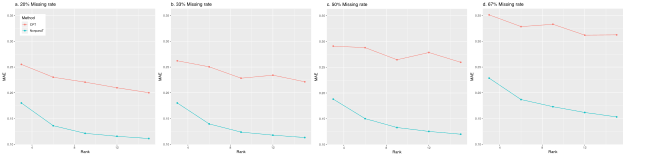
\includegraphics[width = \textwidth]{figure/brain_sim.pdf}
\caption{Estimation error versus rank under different missing rate. Panels (a)-(d) correspond to missing rate 20\%, 33\%, 50\%, and 67\%, respectively. Error bar represents the standard error over 5-fold cross-validations.}\label{fig:braincv}
\end{figure}

We next investigate the pattern in the estimated signal tensor. Figure~\ref{fig:signal} of the main paper shows the identified top edges associated with IQ scores. Specifically, we first obtain a denoised tensor $\hat \Theta\in\mathbb{R}^{68\times 68\times 114}$ using our method with $r=10$ and $H=20$. Then, we perform a regression analysis of $\hat \Theta(i,j,\colon)\in\mathbb{R}^{144}$ against the normalized IQ score across the 144 individuals. The regression model is repeated for each edge $(i,j)\in[68]\times[68]$. We find that top edges represent the interhemispheric connections in the frontal lobes. The result is consistent with the role of interhemispheric connectivity in human intelligence. 

\subsection{NIPS data analysis}
In the main paper we have summarized the MAE in cross-validation experiments for $r=6, 9,12$. Here we provide additional results for a wider range $r= 3, 6, \ldots,15$. Table~\ref{tab:NIPS} suggests that further increment of rank appears to have little effect on the performance. In addition, we also perform naive imputation where the missing values are predicted using the sample average. The two tensor methods outperform the naive imputation, implying the necessity of incorporating tensor structure in the analysis.
\begin{table}[h!]
\centering
\begin{tabular}{c|ccccc}
Method & $r = 3$ & $r = 6$ & $r=9$ & $r=12$&$r=15$ \\
\hline
NonparaT (Ours) & {\bf 0.18}(0.002) & {\bf 0.16}(0.002) & {\bf 0.15}(0.001)& {\bf 0.14}(0.001)&{\bf 0.13}(0.001)\\
 \hline
Low-rank CPT &0.22(0.004) & 0.20(0.007) & 0.19(0.007)&0.17(0.007)&0.17(0.007)\\
  \hline
Naive imputation& \multicolumn{5}{c}{0.32(.001)}\\
\end{tabular}
\caption{Prediction accuracy measured in MAE in the NIPS data analysis. The reported MAEs are averaged over five runs of cross-validation, with standard errors in parentheses. Bold numbers indicate the minimal MAE among three methods. For low-rank CPT, we use R function {\tt rTensor} with default hyperparameters, and for our method, we set $H=20$. }\label{tab:NIPS}
\end{table}



\bibliographystyle{chicago}

\bibliography{tensor_wang}

\end{document}
